\documentclass[11pt]{article}
\usepackage[legalpaper, landscape, margin=1in]{geometry}
\usepackage{mathtools, amsthm, amssymb, amsmath}
\usepackage{multicol}
\usepackage{graphicx}
\graphicspath{{./picture/}}
\usepackage{subcaption}
\usepackage{tikz}
\usetikzlibrary{positioning}
\usepackage{rotating}
\usepackage{mfirstuc}

\begin{document}

\begin{figure}
\centering
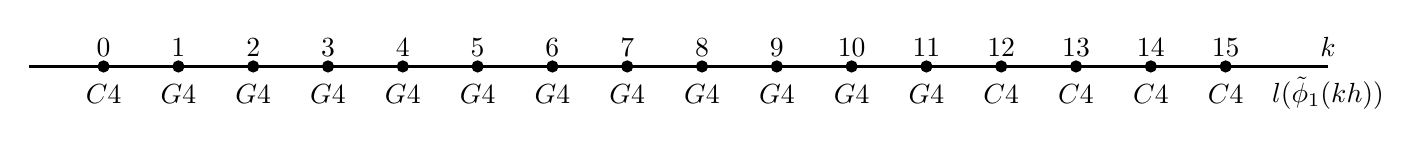
\begin{tikzpicture}
  % Draw number line
  \draw[-, thick] (0,0) -- (16.5,0) node[below] {$l(\tilde{\phi}_1(kh))$}  node[above] {$k$};

  % Data
  \foreach \i/\x/\p in {1/C4/0, 2/G4/1, 3/G4/2, 4/G4/3, 5/G4/4, 6/G4/5, 7/G4/6, 8/G4/7, 9/G4/8, 10/G4/9, 11/G4/10, 12/G4/11, 13/C4/12, 14/C4/13, 15/C4/14, 16/C4/15} {
    % Draw points and labels
    \filldraw (\i*0.95,0) circle (2pt) node[above] {$\p$};
    
    % Draw number scale below the line
    \draw (\i*0.95,-0.1) node[below] {$\x$};
  }

\end{tikzpicture}
\end{figure}





\iffalse
\begin{figure}
\centering

\begin{subfigure}{\textwidth}
  \centering
  \small{
  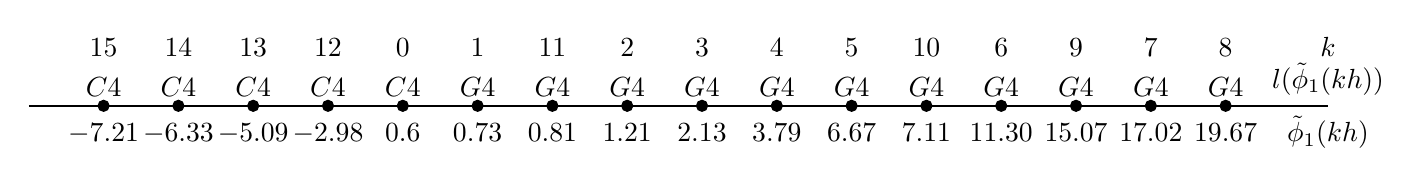
\begin{tikzpicture}
    % Draw number line
    \draw[-, thick] (0,0) -- (16.5,0) node[below] {$\tilde{\phi}_1(kh)$}  node[above] {$l(\tilde{\phi}_1(kh))$} node[above=0.5cm] {$k$};

    % Data
    \foreach \i/\x/\p in {1/-7.21/C4, 2/-6.33/C4, 3/-5.09/C4, 4/-2.98/C4, 5/0.6/C4, 6/0.73/G4, 7/0.81/G4, 8/1.21/G4, 9/2.13/G4, 10/3.79/G4, 11/6.67/G4, 12/7.11/G4, 13/11.30/G4, 14/15.07/G4, 15/17.02/G4, 16/19.67/G4} {
      % Draw points and labels
      \filldraw (\i*0.95,0) circle (2pt) node[above] {$\p$};
      
      % Draw number scale below the line
      \draw (\i*0.95,-0.1) node[below] {$\x$};
    }
    
    % Display the sequence at each point
    \foreach \i/\x in {1/15, 2/14, 3/13, 4/12, 5/0, 6/1, 7/11, 8/2, 9/3, 10/4, 11/5, 12/10, 13/6, 14/9, 15/7, 16/8} {
      \draw (\i*0.95,0.5) node[above] {\x};
    }
  \end{tikzpicture}}
  \caption{For each component in $\{\tilde{\phi}_1(kh)\}_{k=0}^{15}$, apply the $l(\tilde{\phi}_1(kh))$ mapping.}
  \label{subfig2:traj2nmp}

\end{subfigure}

\vspace{5pt}

\begin{subfigure}{\textwidth}
  \centering
  \small{
  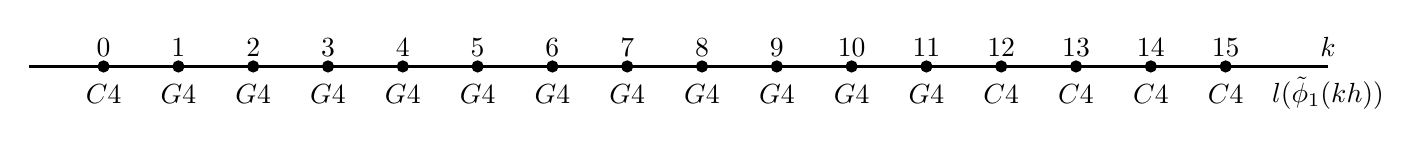
\begin{tikzpicture}
    % Draw number line
    \draw[-, thick] (0,0) -- (16.5,0) node[below] {$l(\tilde{\phi}_1(kh))$}  node[above] {$k$};

    % Data
    \foreach \i/\x/\p in {1/C4/0, 2/G4/1, 3/G4/2, 4/G4/3, 5/G4/4, 6/G4/5, 7/G4/6, 8/G4/7, 9/G4/8, 10/G4/9, 11/G4/10, 12/G4/11, 13/C4/12, 14/C4/13, 15/C4/14, 16/C4/15} {
      % Draw points and labels
      \filldraw (\i*0.95,0) circle (2pt) node[above] {$\p$};
      
      % Draw number scale below the line
      \draw (\i*0.95,-0.1) node[below] {$\x$};
    }

  \end{tikzpicture}}
  \caption{The new variation of the first 16 pitches are marked below the 1D axis.}
  \label{subfig2:nmp}

\end{subfigure}

\caption{The figure for visualizes how a chaotic mapping with melodic variation method can be used to generate musical variations}
\label{fig2:dabbymv method}
\end{figure}
\fi

\end{document}